\documentclass[document.tex]{subfiles}
\begin{document}

\chapter{Literature Review}

\section{Introduction}
\noindent Relevant feature identification has become an essential task to apply data mining algorithms effectively in real-world scenarios. Therefore, many feature selection methods have been proposed to obtain the relevant feature or feature subsets in the literature to achieve their objectives of classification and clustering.
The amount of high-dimensional data that exists and is publically available on the internet has greatly increased in the past few years. Therefore, machine learning methods have difficulty in dealing with the large number of input features, which is posing an interesting challenge for researchers. In order to use machine learning methods effectively,pre-processing of the data is essential. Feature selection is one of the most frequent and important techniques in data pre-processing\cite{2}, and has become an indispensable component of the machine learning process. It is also known as variable selection, attribute selection, or variable subset selection in machine learning and statistics. It is the process of detecting relevant features and removing irrelevant, redundant, or noisy data. This process speeds up data mining algorithms, improves predictive accuracy, and increases
comprehensibility. Irrelevant features are those that provide no useful information, and
redundant features provide no more information than the currently selected features.
\section{Feature Mining}
Hyperspectral sensors record the reflectance from the Earth's surface over the full range of solar wavelengths with high spectral resolution. The resulting high-dimensional data contain rich information for a wide range of applications. However, for a specific application, not all the measurements are important and useful. The original feature space may not be the most effective space for representing the data. Feature mining\cite{33}, which includes feature generation, feature selection (FS), and feature extraction (FE)\cite{5}, is a critical task for hyperspectral data classification. Significant research effort has focused on this issue since hyperspectral data became available in the late 1980s. The feature mining techniques which have been developed include supervised and unsupervised, parametric and nonparametric, linear and nonlinear methods, which all seek to identify the informative subspace.In the process of feature mining, irrelevant and redundant features or noise in the data
may be hinder in many situations, because they are not relevant and important with respect to the class concept such as microarray data analysis . When the number of samples
is much less than the features, then machine learning gets particularly difficult, because
the search space will be sparsely populated. Therefore, the model will not able to differentiate accurately between noise and relevant data . There are two major approaches to
feature selection. The first is Individual Evaluation, and the second is Subset Evaluation.
Ranking of the features is known as Individual Evaluation . In Individual Evaluation,
the weight of an individual feature is assigned according to its degree of relevance. In
Subset Evaluation, candidate feature subsets are constructed using search strategy. The
general procedure for feature selection has four key steps as shown in Figure 3.1
\begin{itemize}
	\item Subset Generation
	\item Evaluation of Subset
	\item Stopping Criteria
	\item Result Validation
\end{itemize}

\begin{figure}[H]
	\begin{center}
		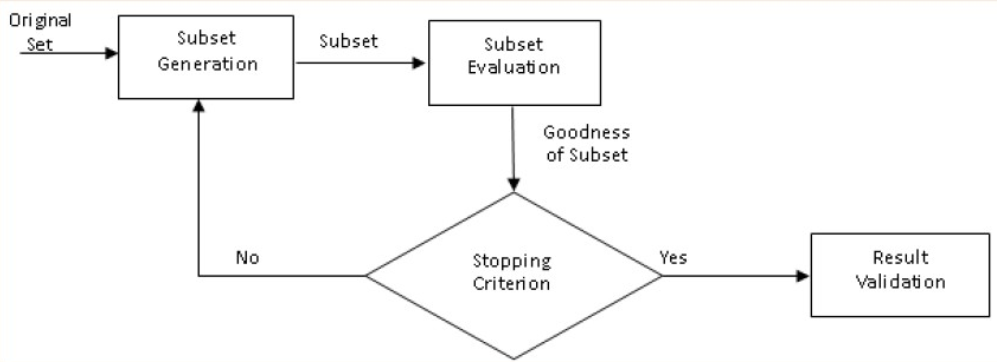
\includegraphics[height=5.0cm]{imgs/Feature_mining.png}
	\end{center}
	\caption{Four key steps for the feature selection process}
	\label{fig:Four key steps for the feature selection process}
\end{figure}
\noindent Subset generation is a heuristic search in which each state specifies a candidate subset
for evaluation in the search space. Two basic issues determine the nature of the subset
generation process. First, successor generation decides the search starting point, which
influences the search direction. To decide the search starting points at each state, forward,
backward, compound, weighting, and random methods may be considered . Second,
search organization is responsible for the feature selection process with a specific strategy,
such as sequential search, exponential search or random search . A newly generated subset
must be evaluated by a certain evaluation criteria. Therefore, many evaluation criteria
have been proposed in the literature to determine the goodness of the candidate subset
of the features. Base on their dependency on mining algorithms, evaluation criteria can
be categorized into groups: independent and dependent criteria . Independent criteria
exploit the essential characteristics of the training data without involving any mining
algorithms to evaluate the goodness of a feature set or feature. And dependent criteria
involve predetermined mining algorithms for feature selection to select features based
on the performance of the mining algorithm applied to the selected subset of features.
Finally, to stop the selection process, stop criteria must be determined. Feature selection
process stops at validation procedure. It is not the part of feature selection process, but
feature selection method must be validate by carrying out different tests and comparisons
with previously established results or comparison with the results of competing methods
using artificial datasets, real world datasets, or both.
The relationship between the inductive learning method and feature selection algorithm
infers a model. There are three general approaches for feature selection. First, the Filter
Approach exploits the general characteristics of training data with independent of the
mining algorithm. Second, the Wrapper Approach explores the relationship between
relevance and optimal feature subset selection\cite{12}. It searches for an optimal feature subset
adapted to the specific mining algorithm. And third, the Embedded Approach is
done with a specific learning algorithm that performs feature selection in the process of
training.
\section{Related Works}
\noindent Many feature selection methods have been proposed in the literature, and their comparative study is a very difficult task. Without knowing the relevant features in advance of
the real data set, it is very difficult to find out the effectiveness of the feature selection
methods, because data sets may include many challenges such as the huge number of irrelevant and redundant features, noisy data, and high dimensionality in term of features
or samples. Therefore, the performance of the feature selection method relies on the performance of the learning method. There are many performance measures mentioned in
the literature such as accuracy, computer resources, ratio of feature selection, etc. Most
researchers agree that there is no so-called "best method". Therefore, the new feature
selection methods are constantly increasing to tackle the specific problem (as mentioned
above) with different strategy.
\begin{itemize}
	\item To ensure a better behavior of feature selection using an ensemble method
	\item Combining with other techniques such as tree ensemble and feature extraction\cite{4}
	\item Reinterpreting existing algorithms
	\item Creating a new method to deal with still-unresolved problems
	\item To combine several feature selection methods
\end{itemize}
Dimensionality reduction prior to classification is advantageous in hyperspectral data
analysis because the dimensionality of the input space greatly affects the performance of
many supervised classification methods\cite{13}. Further, there is a high likelihood of redundancy in the features and it is possible that some features contain less discriminatory
information than others. Moreover, the high-dimensionality imposes requirements for
storage space and computational load. The analysis in \cite{1} supports this line of reasoning
and suggests that feature selection may be a valuable procedure in preprocessing hyperspectral data for classification by the widely used SVM classifier. In hyperspectral
image analysis, feature selection is preferred over feature extraction for dimensionality
reduction \cite{4}, \cite{13}. Feature extraction methods involve transforming the data and hence,
crucial and critical information may be compromised and distorted. In contrast, feature
selection methods strive to discover a subset of features which capture the fundamental
characteristics of the data, while possessing sufficient capacity to discriminate between
classes. Hence, they have the advantage of preserving the relevant original information of
the data. There are various studies which establish the usefulness of feature selection in
hyperspectral data classification. There are various feature selection methods for hyperspectral data such as the SVM Recursive Feature Elimination (SVM-RFE), Correlation
based Feature Selection(CFS), Minimum Redundancy Maximum Relevance(MRMR)
\cite{14} feature selection and Random Forests\cite{15} in current literature. In \cite{5}, a band prioritization scheme based
on Principal Component Analysis (PCA) and classification criterion is presented. Mutual
information is a widely used quantity in various feature selection methods. In \cite{16} and \cite{17} uses mutual information to extract most informative features from the original huge data set. In a general
setting, features are ranked based on the mutual information between the spectral bands
and the reference map(also known as the ground truth). In \cite{10}, mutual information is
computed using the estimated reference map obtained by using available a priori knowledge about the spectral signature of frequently-encountered materials. In \cite{9}, normalized mutual information is computed between class reference and the bands obtained via PCA to select relevant features for better classification accuracy.  

\section{Feature Relevancy and Redundancy}
The optimal feature subset is a subset of all relevant features. Therefore, the relevance
of the features must be properly defined according to their relevance. In the literature,
features are classified by their relevancy with three qualifiers: irrelevant, weakly relevant,
and strongly relevant. A graphical representation is shown in Figure 3.2. Many definitions
have been proposed to answer a question "relevant to what?". In \cite{9}, a greedy search approach is applied to select the most relevant and less redundant features to the class labels. 

	\begin{figure}[H]
	\begin{center}
		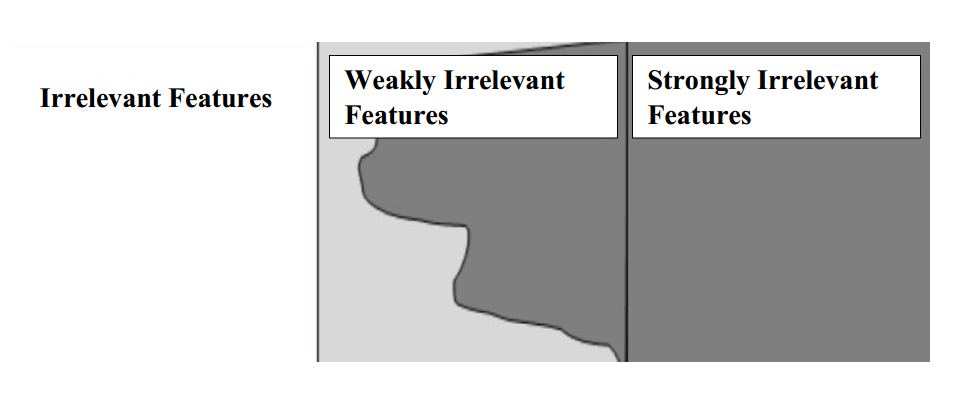
\includegraphics[height=6.0cm]{imgs/relevance.png}
	\end{center}
	\caption{ A view of feature relevance}
	\label{fig: A view of feature relevance}
    \end{figure}

\section{General Approach for Feature Selection}
\noindent The feature selection methods are typically presented in three classes based on how they combine the selection algorithm and the model building.
\begin{enumerate}
	\item \textbf{Filter method: }Filter type methods select variables regardless of the model. They are based only on general features like the correlation with the variable to predict. Filter methods suppress the least interesting variables. The other variables will be part of a classification or a regression model used to classify or to predict data. These methods are particularly effective in computation time and robust to overfitting.
	\begin{figure}[H]
		\begin{center}
			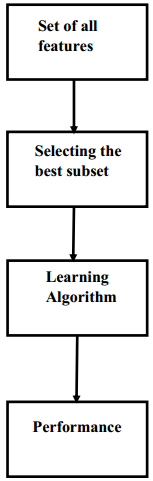
\includegraphics[height=1.0cm]{imgs/filterMethod.png}
		\end{center}
		\caption{Filter Method for feature selection}
		\label{fig:Filter Method for feature selection}
	\end{figure}
	However, filter methods tend to select redundant variables because they do not consider the relationships between variables. Therefore, they are mainly used as a pre-process method.
	\item \textbf{Wrapper method:} Wrapper methods evaluate subsets of variables which allows, unlike filter approaches, to detect the possible interactions between variables. The two main disadvantages of these methods are :
	\begin{itemize}
		\item The increasing overfitting risk when the number of observations is insufficient.
		\item The significant computation time when the number of variables is large.
	\end{itemize}
	\begin{figure}[H]
		\begin{center}
			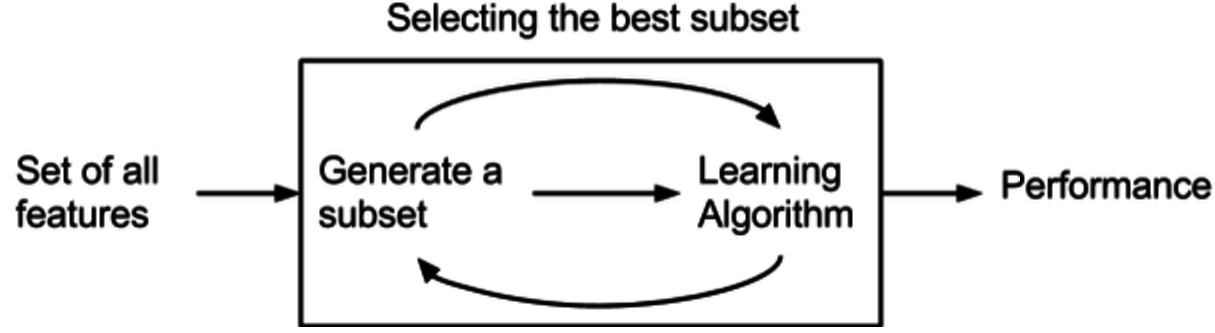
\includegraphics[height=3.0cm]{imgs/wrapperMethod.png}
		\end{center}
		\caption{Wrapper Method for Feature selection}
		\label{fig:Wrapper Method for Feature selection}
	\end{figure}

	\item \textbf{Embedded method:} Embedded methods have been recently proposed that try to combine the advantages of both previous methods. A learning algorithm takes advantage of its own variable selection process and performs feature selection and classification simultaneously.
	\begin{figure}[H]
		\begin{center}
			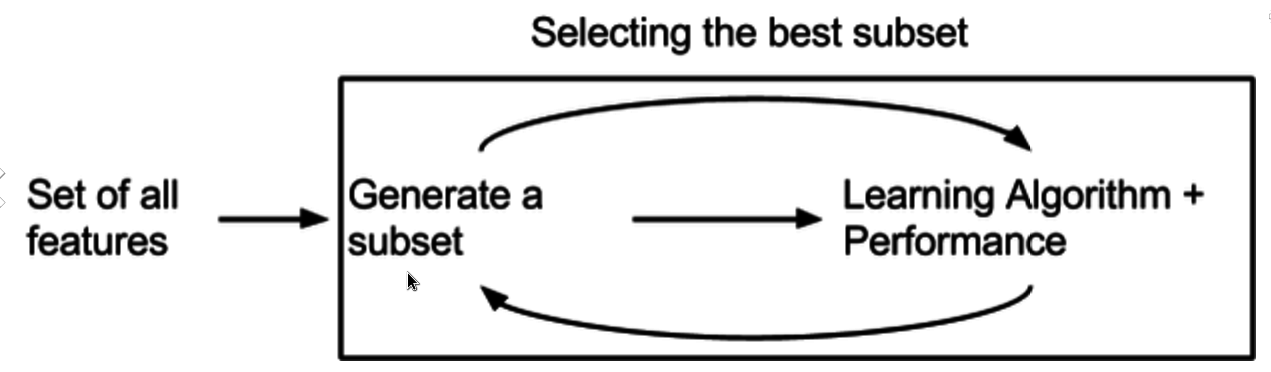
\includegraphics[height=3.0cm]{imgs/embeddedMethod.png}
		\end{center}
		\caption{Embedded Method for Feature selection}
		\label{fig:Embedded Method for Feature selection}
	\end{figure}
\end{enumerate}
\section{Feature Mining for Hyperspectral Image}
\noindent Hyperspectral sensors record the reflectance from the Earth’s surface over the full range
of solar wavelengths with high spectral resolution. The resulting high dimensional data
contain rich information for a wide range of applications. However, for a specific application, not all the measurements are important and useful. The original feature space may
not be the most effective space for representing the data. Feature mining, which includes
feature generation, feature selection (FS), and feature extraction (FE), is a critical task
\begin{figure}[H]
	\begin{center}
		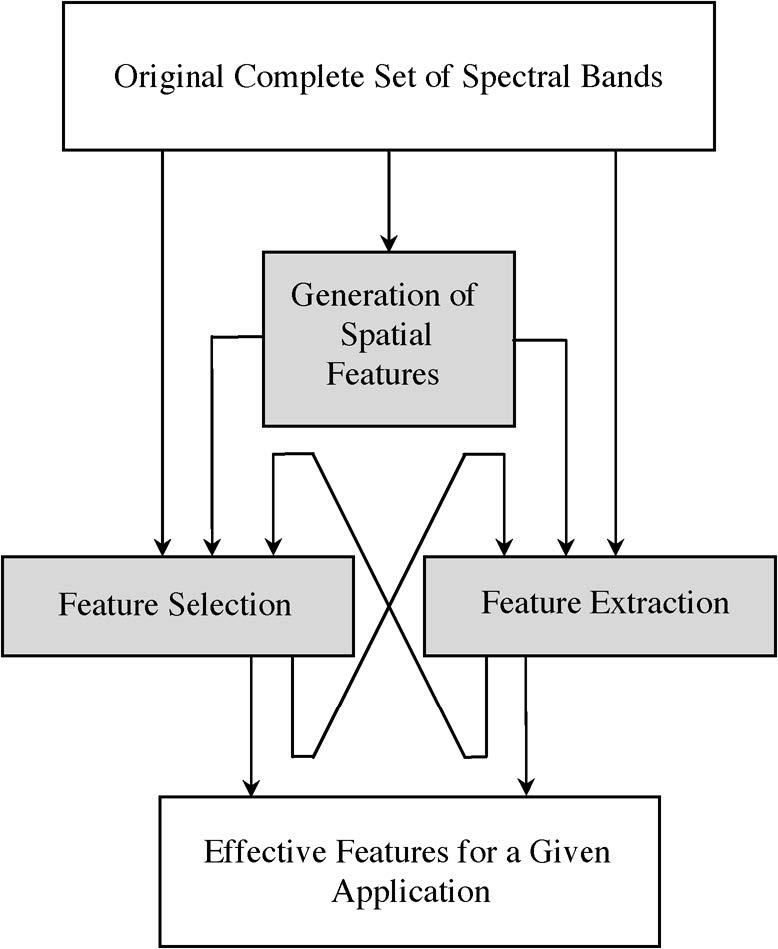
\includegraphics[height=6.0cm]{imgs/OperationFeatureMining.png}
	\end{center}
	\caption{Possible operations for feature mining (only one path is used for any specific
		approach).}
	\label{fig:Possible operations for feature mining (only one path is used for any specific
		approach).}
\end{figure}
for hyperspectral data classification. Significant research effort has focused on this issue since hyperspectral data became available in the late 1980s. The feature mining techniques which have been developed include supervised and unsupervised, parametric and
nonparametric, linear and nonlinear methods, which all seek to identify the informative
subspace. This paper provides an overview of both conventional and advanced feature
reduction methods, with details on a few techniques that are commonly used for analysis
of hyperspectral data. A general form that represents several linear and nonlinear FE
methods is also presented. Experiments using two widely available hyperspectral data
sets are included to illustrate selected FS and FE methods.

\section{Classification Techniques}
\noindent Digital image classification techniques group pixels to represent land cover features. Land cover could be forest, urban, agricultural and other types of features. There are two main image classification techniques.
\begin{itemize}
	\item Unsupervised Classification
	\item Supervised Classification
\end{itemize}
\subsection{Unsupervised Classification}
\noindent Pixels are grouped based on the reflectance properties of pixels. These groupings are
called "clusters". The user identifies the number of clusters to generate and which bands
to use. With this information, the image classification software generates clusters. There
are different image clustering algorithms such as K-means and ISODATA.
Unsupervised classification is a method which examines a large number of unknown pixels and divides into a number of classed based on natural groupings present in the image values. unlike supervised classification, unsupervised classification does not require
analyst-specified training data. The basic premise is that values within a given cover
type should be close together in the measurement space (i.e. have similar gray levels),
whereas data in different classes should be comparatively well separated (i.e. have very
different gray levels) (PCI, 1997; Lillesand and Kiefer, 1994; Eastman, 1995 )
The classes that result from unsupervised classification are spectral classed which based on natural groupings of the image values, the identity of the spectral class will not be initially known, must compare classified data to some from of reference data (such as larger
scale imagery, maps, or site visits) to determine the identity and informational values
of the spectral classes. Thus, in the supervised approach, to define useful information
categories and then examine their spectral separability; in the unsupervised approach the
computer determines spectrally separable class, and then define their information value.
(PCI, 1997; Lillesand and Kiefer, 1994)

\begin{figure}[H]
	\begin{center}
		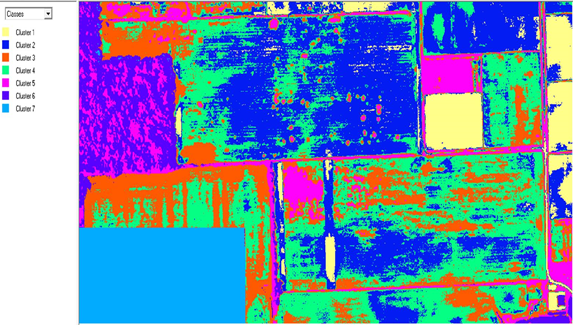
\includegraphics[height=6.0cm]{imgs/Unsupervised.png}
	\end{center}
	\caption{Unsupervised Classification}
	\label{fig: Unsupervised Classification}
\end{figure}
Unsupervised classification is becoming increasingly popular in agencies involved in
long term GIS database maintenance. The reason is that there are now systems that use
clustering procedures that are extremely fast and require little in the nature of operational parameters. Thus it is becoming possible to train GIS analysis with only a general
familiarity with remote sensing to undertake classifications that meet typical map accuracy standards. With suitable ground truth accuracy assessment procedures, this tool can provide a remarkably rapid means of producing quality land cover data on a continuing basis.

\subsection{Supervised Classification}
\noindent The user selects representative samples for each land cover class in the digital image.
These sample land cover classes are called "training sites". The image classification
software uses the training sites to identify the land cover classes in the entire image.
The classification of land cover is based on the spectral signature defined in the training set. The digital image classification software determines each class on what it resembles
\begin{figure}[H]
	\begin{center}
		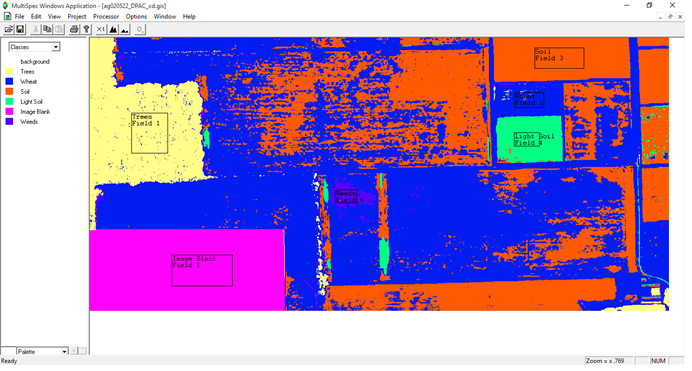
\includegraphics[height=6.0cm]{imgs/Supervised.png}
	\end{center}
	\caption{Supervised Classification}
	\label{fig: Supervised Classification}
\end{figure}
most in the training set. The common supervised classification algorithms are maximum
likelihood\cite{19} and support vector machine\cite{18}.
\end{document}